\documentclass[conference]{IEEEtran}

\usepackage[T1]{fontenc}
\usepackage{graphicx}
\usepackage{amsmath,amssymb}
\usepackage{booktabs}
\usepackage{cleveref}
\usepackage[backend=biber,style=ieee]{biblatex}
\addbibresource{refs.bib}

\begin{document}

\title{How Robust Is Character-Level Transliteration to Informal Typing?\\
A Paired Noise Benchmark for Romanized Tamil}

\author{\IEEEauthorblockN{Lebi Raja}
\IEEEauthorblockA{Department of AI \& Data Science\\
Karunya Institute of Technology and Sciences, India}}

\maketitle

\begin{abstract}
Tamil speakers routinely type Tamil in Latin letters (``Tanglish'') and software must convert it back to Tamil script.
Published transliteration models are trained and tested on carefully romanized text, so their behaviour on hurried, informal typing is largely unmeasured.
We study this gap for word-level Latin-to-Tamil transliteration with character-level sequence-to-sequence models.
We contribute (i)~a paired robustness benchmark that applies seven Tamil-specific noise operators at four severities to the Dakshina test lexicon, so every noisy input is tied to its clean form and gold answer, together with a real-chat word set and a team-typed set;
(ii)~an augmentation study comparing random character noise, Tamil-phonological noise and sampled back-transliteration against a more-data control;
and (iii)~a parameter-matched comparison of a BiLSTM with attention and a small pre-LN Transformer, with five seeds and equal tuning budget.
Our implementation reproduces the published Dakshina baselines within one CER point.
Results of the benchmark and the augmentation study are reported in Section~\ref{sec:results}.
\end{abstract}

\begin{IEEEkeywords}
transliteration, Tamil, robustness, data augmentation, sequence-to-sequence, romanization
\end{IEEEkeywords}

\section{Introduction}
Most Tamil speakers type on phones using the Latin alphabet.
Search, autocomplete and display all need the text converted back into Tamil script, which is a transliteration task: sounds are mapped to letters, not meanings to words.
The Latin alphabet cannot express several Tamil distinctions, including vowel length, doubled consonants and the several n, l and r sounds, and writers spell the same word in different ways.
Informal typing adds more variation: dropped vowels (\emph{kankl} for \emph{kanakkil}), collapsed long vowels, collapsed doubled consonants, swapped digraphs and stretched letters.

Neural transliteration is well studied on clean data.
The Dakshina dataset provides romanizations of Tamil words written by native speakers on request~\cite{roark2020dakshina}, and strong systems have been trained on larger corpora~\cite{madhani2023aksharantar}.
However, the Tamil text in Dakshina is encyclopaedic and was typed carefully, so it does not contain the shorthand found in chat.
We therefore ask how much character-level models lose under informal typing, which training strategy recovers it, and whether the choice of architecture matters.

The literature also disagrees on architecture.
On Dakshina Tamil, an LSTM beat a Transformer in one study~\cite{roark2020dakshina}, whereas a Transformer was better in another~\cite{kirov2024context}, and batch size can reverse the ranking~\cite{wu2021applying}.
None of these comparisons tested noisy input.

\textbf{Contributions.}
(1)~A paired, seeded robustness benchmark for Tamil with seven noise operators and four severities.
(2)~A study of four augmentation strategies and a more-data control, evaluated on held-out noise types and on real typing.
(3)~A parameter-matched, equal-tuning comparison of BiLSTM-attention and Transformer over five seeds with paired significance tests.
(4)~A reproducibility package: code, configurations, per-run logs and data checksums.

\section{Related Work}
\textbf{Transliteration datasets and systems.}
Dakshina covers twelve South Asian languages with native-script Wikipedia text, a romanization lexicon and romanized sentences~\cite{roark2020dakshina}.
Aksharantar and the IndicXlit model extend coverage to 21 languages with millions of pairs~\cite{madhani2023aksharantar}.
Earlier systems include Brahmi-Net~\cite{kunchukuttan2015brahminet} and the shared tasks collected in NEWS~\cite{chen2018news}.
Context-aware and large-model approaches have recently been compared with character models~\cite{kirov2024context,azam2025beyond}.

\textbf{Noisy and informal romanization.}
Keyboard data show how users romanize at scale~\cite{hellsten2017keyboard}, and a large study documents Latin-script variation across South Asian languages~\cite{wolfsonkin2019latin}.
For Tamil, a shorthand-aware study examines vowel dropping but evaluates no neural model~\cite{herath2024tamzhi}, and a Malayalam study reports CER rising from 7.4 to 22.7 when vowels are dropped~\cite{baiju2024malayalam}.
Code-mixed Tamil corpora provide real informal text without Tamil-script labels~\cite{chakravarthi2020tamilmix}.

\textbf{Robustness and augmentation.}
Character models are brittle to noise unless trained with it~\cite{belinkov2018synthetic}, and mixing noise types helps~\cite{karpukhin2019training}.
Synthetic variation improves romanized language identification~\cite{benton2025romanizedlid}, and sampled back-translation is a standard way to create synthetic parallel data~\cite{sennrich2016backtranslation}.
We transfer these ideas to Tamil transliteration.

\textbf{Evaluation practice.}
Parameter confounds and weak statistics can reverse conclusions in character-level transduction~\cite{moran2020effective}; we match model size and tuning budget and report seed variance.

\section{Data and Benchmark}
\label{sec:data}
% System architecture figure (hand-drawn TikZ; included from sections/method.tex).
% Source of truth for the shapes: src/translit/models.py (TransformerS2S), noise.py (OPS),
% augment.py (conditions A0-A4, CTRL), decode.py (beam_search), finetune.py (v2 deployment model).
\begin{figure*}[t]
\centering
\resizebox{\textwidth}{!}{%
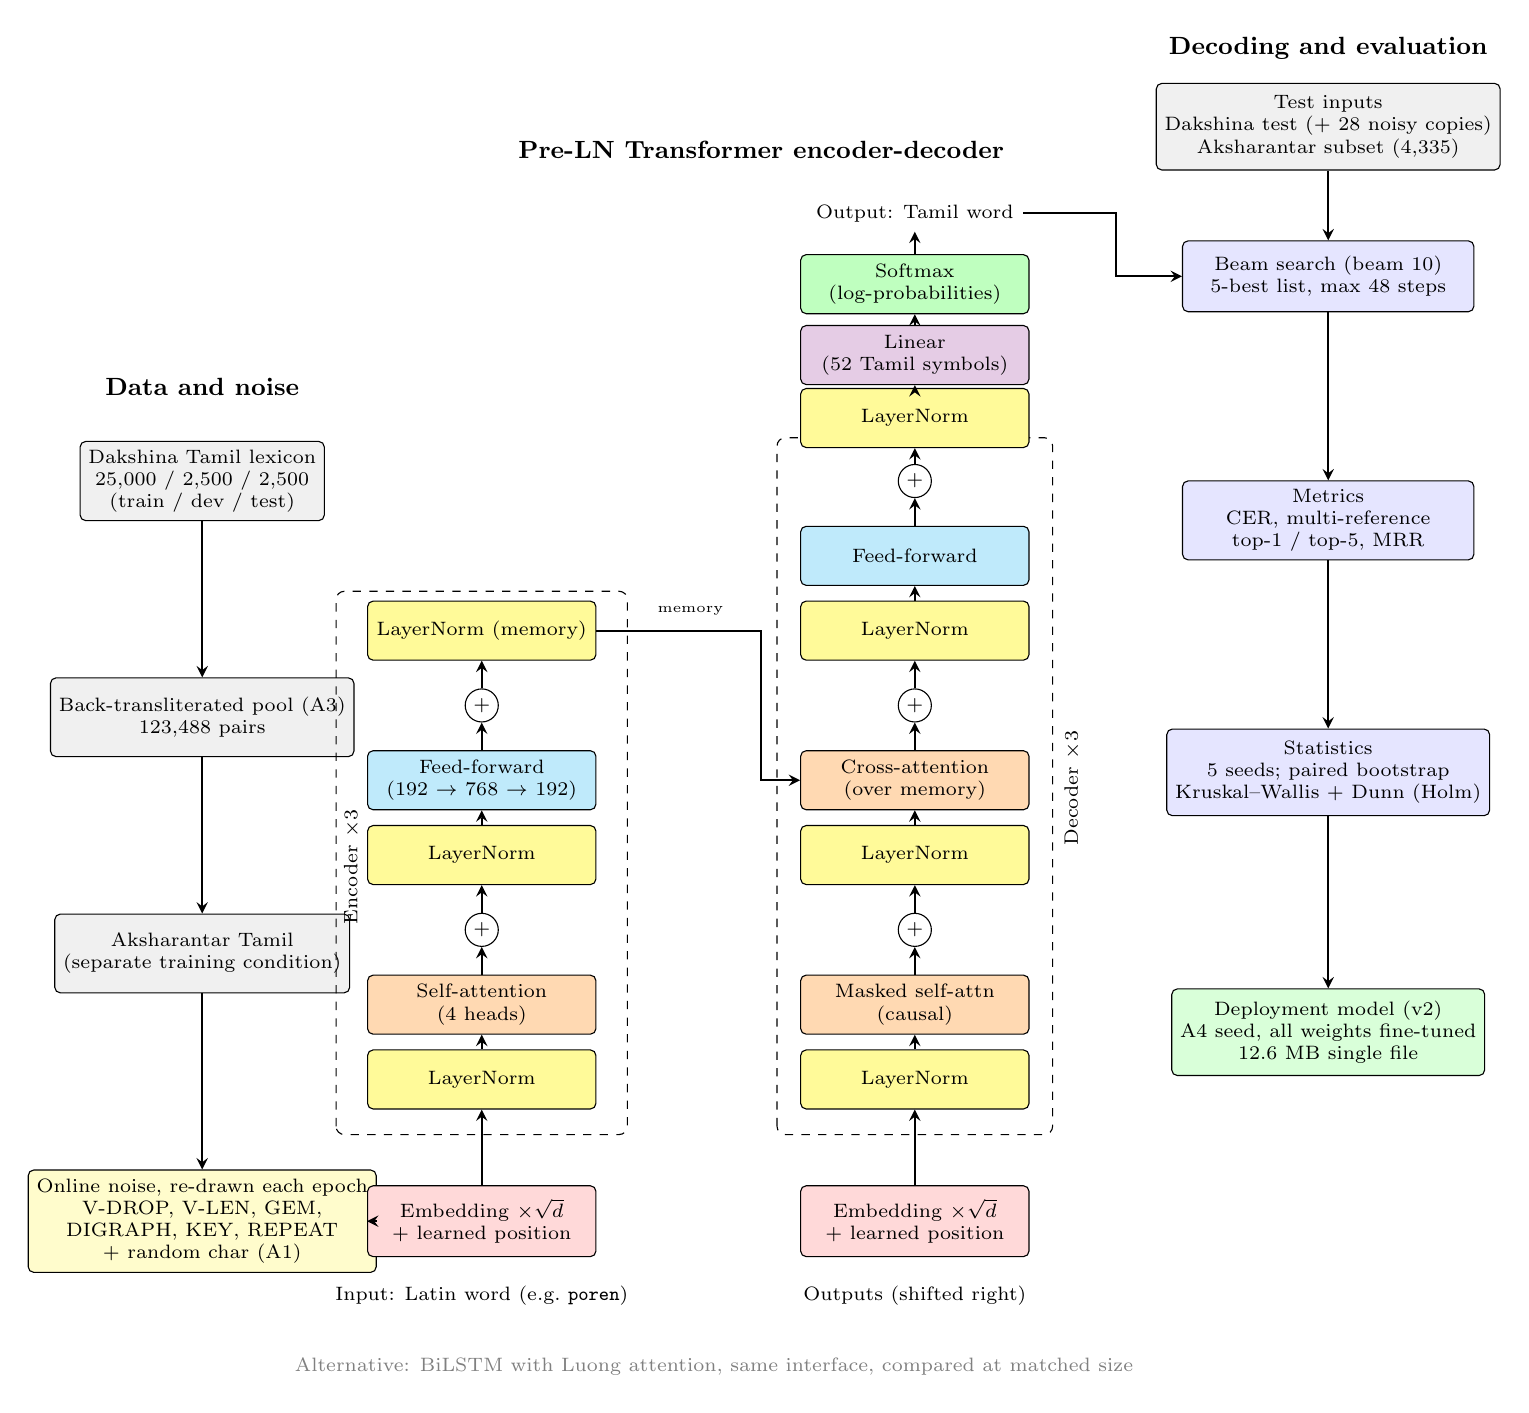
\begin{tikzpicture}[
  blk/.style={draw, rounded corners=2pt, minimum width=2.9cm, minimum height=0.75cm, font=\scriptsize, align=center, inner sep=3pt},
  emb/.style={blk, fill=red!15, minimum height=0.9cm},
  att/.style={blk, fill=orange!30},
  ffn/.style={blk, fill=cyan!25},
  nrm/.style={blk, fill=yellow!40},
  outp/.style={blk, fill=violet!20},
  smx/.style={blk, fill=green!25},
  dat/.style={blk, minimum width=3.0cm, fill=gray!12, minimum height=1.0cm},
  add/.style={circle, draw, inner sep=0pt, minimum size=0.42cm, font=\scriptsize},
  grp/.style={draw, dashed, rounded corners=3pt},
  arr/.style={->, >=stealth, thick},
]

% ---------- Column A: data and noise ----------
\node[font=\small\bfseries] at (1.5,11.6) {Data and noise};
\node[dat] (a1) at (1.5,10.4) {Dakshina Tamil lexicon\\25{,}000 / 2{,}500 / 2{,}500\\(train / dev / test)};
\node[dat] (a2) at (1.5,7.4) {Back-transliterated pool (A3)\\123{,}488 pairs};
\node[dat] (a3) at (1.5,4.4) {Aksharantar Tamil\\(separate training condition)};
\node[dat, minimum height=1.3cm, fill=yellow!20] (a4) at (1.5,1.0) {Online noise, re-drawn each epoch\\V-DROP, V-LEN, GEM,\\DIGRAPH, KEY, REPEAT\\+ random char (A1)};
\draw[arr] (a1) -- (a2);
\draw[arr] (a2) -- (a3);
\draw[arr] (a3) -- (a4);

% ---------- Column B: Transformer encoder-decoder ----------
\node[font=\small\bfseries] at (8.6,14.6) {Pre-LN Transformer encoder-decoder};

% Encoder (source = romanized word)
\node[emb] (e1) at (5.05,1.0) {Embedding $\times\sqrt{d}$\\+ learned position};
\node[nrm] (e2) at (5.05,2.8) {LayerNorm};
\node[att] (e3) at (5.05,3.75) {Self-attention\\(4 heads)};
\node[add] (e4) at (5.05,4.7) {$+$};
\node[nrm] (e5) at (5.05,5.65) {LayerNorm};
\node[ffn] (e6) at (5.05,6.6) {Feed-forward\\(192 $\rightarrow$ 768 $\rightarrow$ 192)};
\node[add] (e7) at (5.05,7.55) {$+$};
\node[nrm] (en) at (5.05,8.5) {LayerNorm (memory)};
\draw[grp] (3.2,2.1) rectangle (6.9,9.0);
\node[rotate=90, font=\scriptsize] at (3.4,5.5) {Encoder $\times 3$};
\draw[arr] (e1) -- (e2);
\draw[arr] (e2) -- (e3);
\draw[arr] (e3) -- (e4);
\draw[arr] (e4) -- (e5);
\draw[arr] (e5) -- (e6);
\draw[arr] (e6) -- (e7);
\draw[arr] (e7) -- (en);

% Decoder (target shifted right, causal)
\node[emb] (d1) at (10.55,1.0) {Embedding $\times\sqrt{d}$\\+ learned position};
\node[nrm] (d2) at (10.55,2.8) {LayerNorm};
\node[att] (d3) at (10.55,3.75) {Masked self-attn\\(causal)};
\node[add] (d4) at (10.55,4.7) {$+$};
\node[nrm] (d4n) at (10.55,5.65) {LayerNorm};
\node[att] (d5) at (10.55,6.6) {Cross-attention\\(over memory)};
\node[add] (d6) at (10.55,7.55) {$+$};
\node[nrm] (d7) at (10.55,8.5) {LayerNorm};
\node[ffn] (d8) at (10.55,9.45) {Feed-forward};
\node[add] (d9) at (10.55,10.4) {$+$};
\draw[grp] (8.8,2.1) rectangle (12.3,10.95);
\node[rotate=90, font=\scriptsize] at (12.55,6.5) {Decoder $\times 3$};
\draw[arr] (d1) -- (d2);
\draw[arr] (d2) -- (d3);
\draw[arr] (d3) -- (d4);
\draw[arr] (d4) -- (d4n);
\draw[arr] (d4n) -- (d5);
\draw[arr] (d5) -- (d6);
\draw[arr] (d6) -- (d7);
\draw[arr] (d7) -- (d8);
\draw[arr] (d8) -- (d9);

% Memory from encoder into decoder cross-attention
\draw[arr] (en.east) -- (8.6,8.5) |- (d5.west);
\node[font=\tiny] at (7.7,8.75) {memory};

% Output head
\node[nrm] (of) at (10.55,11.2) {LayerNorm};
\node[outp] (o1) at (10.55,12.0) {Linear\\(52 Tamil symbols)};
\node[smx] (o2) at (10.55,12.9) {Softmax\\(log-probabilities)};
\node[font=\scriptsize] (o3) at (10.55,13.8) {Output: Tamil word};
\draw[arr] (d9) -- (of);
\draw[arr] (of) -- (o1);
\draw[arr] (o1) -- (o2);
\draw[arr] (o2) -- (o3);

% Inputs
\node[font=\scriptsize] at (5.05,0.05) {Input: Latin word (e.g.\ \texttt{poren})};
\node[font=\scriptsize] at (10.55,0.05) {Outputs (shifted right)};
\draw[arr] (a4.east) -- (e1.west);
\node[font=\scriptsize, text=gray] at (8.0,-0.85) {Alternative: BiLSTM with Luong attention, same interface, compared at matched size};

% ---------- Column C: decoding and evaluation ----------
\node[font=\small\bfseries] at (15.8,15.9) {Decoding and evaluation};
\node[dat, minimum height=1.1cm] (t0) at (15.8,14.9) {Test inputs\\Dakshina test (+ 28 noisy copies)\\Aksharantar subset (4{,}335)};
\node[blk, fill=blue!10, minimum width=3.7cm, minimum height=0.9cm] (c1) at (15.8,13.0) {Beam search (beam 10)\\5-best list, max 48 steps};
\node[blk, fill=blue!10, minimum width=3.7cm, minimum height=1.0cm] (c2) at (15.8,9.9) {Metrics\\CER, multi-reference\\top-1 / top-5, MRR};
\node[blk, fill=blue!10, minimum width=3.7cm, minimum height=1.1cm] (c3) at (15.8,6.7) {Statistics\\5 seeds; paired bootstrap\\Kruskal--Wallis + Dunn (Holm)};
\node[blk, fill=green!15, minimum width=3.7cm, minimum height=1.1cm] (c4) at (15.8,3.4) {Deployment model (v2)\\A4 seed, all weights fine-tuned\\12.6 MB single file};
\draw[arr] (t0) -- (c1);
\draw[arr] (c1) -- (c2);
\draw[arr] (c2) -- (c3);
\draw[arr] (c3) -- (c4);
\draw[arr] (o3.east) -- (13.1,13.8) |- (c1.west);

\end{tikzpicture}%
}
\caption{Architecture of the system. Left: the data sources, and the noise that is re-drawn online each epoch (six Tamil-specific operators, plus random character noise for A1). Centre: the pre-LN Transformer encoder-decoder used in the main comparison (three layers per side, four heads, $d{=}192$, feed-forward width 768, learned positions; 3.15M parameters at the deployment size). Each sublayer is LayerNorm, then the sublayer, then the residual addition ($+$); the encoder output passes through a final LayerNorm to the decoder's cross-attention. Right: test inputs are decoded with beam search (beam 10) and scored; statistics use five seeds and paired bootstrap; the best A4 seed is fine-tuned into the deployment model.}
\label{fig:architecture}
\end{figure*}

\textbf{Training and clean evaluation.}
We use the Dakshina Tamil romanization lexicon: 25{,}000 training words (68{,}218 romanization pairs), 2{,}500 development words (6{,}827 pairs) and 2{,}500 test words (6{,}864 pairs), which are word-disjoint~\cite{roark2020dakshina}.
Inputs are lowercase Latin and outputs are NFC-normalised Tamil.
A romanization attested for several native forms is scored against all of them.
The development set is used only for early stopping and tuning.
The test lexicon holds 6{,}833 distinct romanized inputs.

\textbf{Independent test sets.}
Aksharantar's Tamil test file contains every Dakshina test pair~\cite{madhani2023aksharantar}.
We keep only rows whose native word occurs in no Dakshina split, which gives three subsets by source: AK-Freq (2{,}607 distinct inputs, frequent web words), AK-NEI (991) and AK-NEF (706), plus their union AK-all.
We also found that Aksharantar's training file shares stems with Dakshina test words, so we never train on it in the controlled experiments.

\textbf{Paired noisy test sets.}
Seven operators perturb the romanized input only (\Cref{tab:ops}).
Each of the 6{,}833 test inputs is perturbed at severity $p\in\{0.1,0.2,0.3,0.5\}$ with a random seed derived from the word, operator and severity.
The 28 sets are therefore exactly reproducible, and each noisy item stays paired with its clean form and references.
Operators and rates are motivated by the typing phenomena in the literature~\cite{wolfsonkin2019latin,herath2024tamzhi,belinkov2018synthetic}.
The digraph operator swaps in both directions (th$\leftrightarrow$t, dh$\leftrightarrow$d, sh$\leftrightarrow$s, ch$\leftrightarrow$c,s) and maps zh to l or z only one way, because in our own measurement on public code-mixed Tamil comments~\cite{chakravarthi2020tamilmix} (heuristic, unverified by hand) vowel dropping, vowel-length collapse and stretching occur several times more often than in Dakshina, while dropped h does not.
\Cref{tab:ops} reports realised strength: nominal $p$ is a per-position probability, so we report the share of words changed; the character edit rate at $p{=}0.3$ is 12.7\% for V-DROP, 7.4\% for KEY and 15.8\% for MIX (see the repository manifest for all sets).

\begin{table}[t]
\caption{Noise operators and the share of test words they change (\%) at three severities.}
\label{tab:ops}
\centering\footnotesize
\resizebox{\columnwidth}{!}{\begin{tabular}{llccc}
\toprule
Operator & Effect & \multicolumn{3}{c}{Words changed (\%) at $p=$} \\
\cmidrule(lr){3-5}
 & & 0.1 & 0.3 & 0.5 \\
\midrule
V-DROP & delete non-initial vowels & 34 & 73 & 89 \\
V-LEN & collapse doubled vowels & 4 & 13 & 21 \\
GEM & collapse doubled consonants & 3 & 9 & 15 \\
DIGRAPH & th/t, dh/d, sh/s, ch/c/s swaps; zh$\to$l,z & 12 & 32 & 47 \\
KEY & adjacent QWERTY key substitution & 21 & 52 & 69 \\
REPEAT & stretch one vowel by 1--3 letters & 10 & 29 & 51 \\
MIX & random combination of the six & 35 & 69 & 82 \\
\bottomrule
\end{tabular}}
\end{table}

\textbf{Synthetic training data.}
For the augmentation study we construct a pool of 60{,}000 further Tamil words from the IndicXlit unigram list.
We remove every Dakshina word, every independent-test word and any word sharing a five-code-point prefix with a held-out word (46{,}652 of 137{,}748 candidates were removed for stem overlap alone).
A Tamil-to-Latin BiLSTM trained on Dakshina romanizes each pool word three times by sampling at temperature 1; a closeness filter against the model's greedy output drops 17{,}828 degenerate samples and leaves 123{,}488 pairs.
A control set romanizes the same 60{,}000 words once, greedily (60{,}000 pairs).
These romanizations are machine-made, so they carry the errors of the model that made them.

\section{Method}
\label{sec:method}
\textbf{Models.}
Both models are character-level with separate source and target vocabularies built from training data.
The BiLSTM uses a two-layer bidirectional encoder, a two-layer LSTM decoder and Luong general attention~\cite{luong2015effective,bahdanau2015neural}.
The Transformer is a pre-LN encoder-decoder with three layers per side and learned positions~\cite{vaswani2017attention}.
Each architecture is built at about 1M, 3M and 8M trainable parameters by choosing the width.

\textbf{Training and decoding.}
Adam, cross-entropy with optional label smoothing, gradient clipping at 1.0, early stopping on development CER.
Decoding uses beam search with beam 10 to produce an $n$-best list.

\textbf{Metrics.}
CER is the corpus-level Levenshtein distance over code points between the top hypothesis and the closest attested reference, divided by reference length.
Top-$k$ accuracy counts an input correct if any of the best $k$ hypotheses equals any reference; MRR uses the rank of the first correct hypothesis.

\textbf{Augmentation conditions.}
A0: Dakshina only.
A1: random character noise (deletion, insertion, substitution, swap).
A2: the Tamil-phonological operators.
A3: Dakshina plus sampled back-transliteration.
A4: A2 plus A3.
CTRL: Dakshina plus the same pool words romanized greedily, which separates more data from more spelling variation.
Online noise is re-drawn every epoch with 40\% of items left clean; held-out variants of A2 omit one operator and are tested on it.

\textbf{Statistics.}
Five seeds per configuration; mean and standard deviation; paired bootstrap over test items for system pairs; Kruskal--Wallis with Dunn post-hoc for more than two systems; Spearman correlation between synthetic and human-set degradation.

\section{Experimental Setup}
All models are trained with PyTorch 2.11 (CUDA 12.8) on an RTX 5070 (12\,GB).
Hyperparameters are chosen by 20 random-search trials per architecture and size using development CER only; test data are never used for selection.

\textbf{Reproduction check.}
Before any new experiment we verify that our implementation matches published results.
With one seed and 3M parameters, our BiLSTM reaches development CER 8.95 and top-1 62.8\% against 8.4 and 65.3\% reported by Roark et al.~\cite{roark2020dakshina}, and our Transformer reaches CER 9.38 against 9.4.
Both CERs are within one point of the published values; the 2.5-point top-1 gap for the BiLSTM may come from differences in how references are counted and is not hidden.

\section{Results}
\label{sec:results}
Full results (C3 architecture comparison, C1 degradation curves, C2 augmentation, real-typing sets) are produced by the experiment queue on the lab server and will be inserted here from the logged JSON files.
The table and figure templates are fixed in the project plan; no number is reported until it comes from a logged run.

\section{Limitations and Threats to Validity}
\label{sec:limits}
\textbf{No real typing yet.}
All noise is synthetic and applied to Dakshina romanizations, which are formal text typed with care, not chat.
We built a real-chat word set from private message exports and a protocol for a team-typed set.
Only a preliminary check of the real-chat set exists (\Cref{sec:final}) and its labels are not yet verified by a person, and the team-typed set has not been collected, so the question of whether synthetic noise predicts real typing (our RQ2) is open.
We therefore speak of informal \emph{romanized} Tamil and make no claim about chat text.

\textbf{Synthetic noise and training data.}
The operators and their rates come from the literature and from measurements on public code-mixed corpora, not from a hand-checked sample of real typing.
Back-transliterated pairs are machine-made and inherit the errors of the generating model.
Operators in the noisy test sets are the same ones that A2 trains on, except KEY and REPEAT, so only these two measure transfer.

\textbf{Tuning and statistics.}
Hyperparameters were tuned once per architecture and size on clean development CER with one seed, and noise-trained conditions reuse the tuned clean settings; early stopping uses clean development CER, which disadvantages noise-trained models.
Five seeds give low power for small differences, and the paired bootstrap does not model seed variation.
Parameter counts are matched only approximately.

\textbf{An incident.}
A bug in our job supervisor started duplicate worker processes overnight, and 33 of the first 72 finished augmentation runs were trained while a duplicate process trained the same run and shared its checkpoint folder.
We checked the damage three ways.
A clean rerun of one affected BiLSTM run reproduced the stored result exactly; a clean rerun of one affected Transformer run differed slightly (test CER 9.30 against 9.13), which is within normal seed variation for a non-deterministic model; and a per-item re-scoring of all 110 stored checkpoints found one model that did not reproduce its logged score (8.43 against 8.49 CER).
That run was retrained cleanly and all other results were kept; the scripts, logs and the incident report are in the repository.

\textbf{Privacy.}
The real-chat words come from the author's own private conversations with other people.
Only a list of distinct lowercase words with counts was extracted (no messages, names or timestamps), the list stays on the author's machines and was labelled without sender information, and only aggregate scores are reported here.
The data cannot be released.

\textbf{Other.}
Dakshina's Tamil lexicon contains about 0.35\% bad pairs, which we did not remove from the test set.
Vowel-dropped inputs can be genuinely ambiguous, so top-1 accuracy understates what a user-facing system with alternatives achieves.
Our models are word-level; no sentence context is used.


\printbibliography

\end{document}
